% CONSORT flow diagram for the eRegTime trial.
% Based on: https://texample.net/tikz/examples/consort-flowchart/
%
% Compile tfrom .tex to .png using:
% pdflatex eRegTime_CONSORT.tex
%
% Convert to a high-res PNG using:
% sips -s format png --resampleWidth 10000 eRegTime_CONSORT.pdf --out eRegTime_CONSORT.png

\documentclass{article}
\usepackage[latin1]{inputenc}
\usepackage{tikz}
\usetikzlibrary{shapes,arrows}
\usepackage{enumitem}

\newcommand*{\h}{\hspace{5pt}}% for indentation
\newcommand*{\hh}{\h\h}% double indentation

\begin{document}
\pagestyle{empty}
\pagecolor{white}
\begin{center}
  % setting the typeface to sans serif and the font size to small
  % the scope local to the environment
  \sffamily
  \footnotesize
  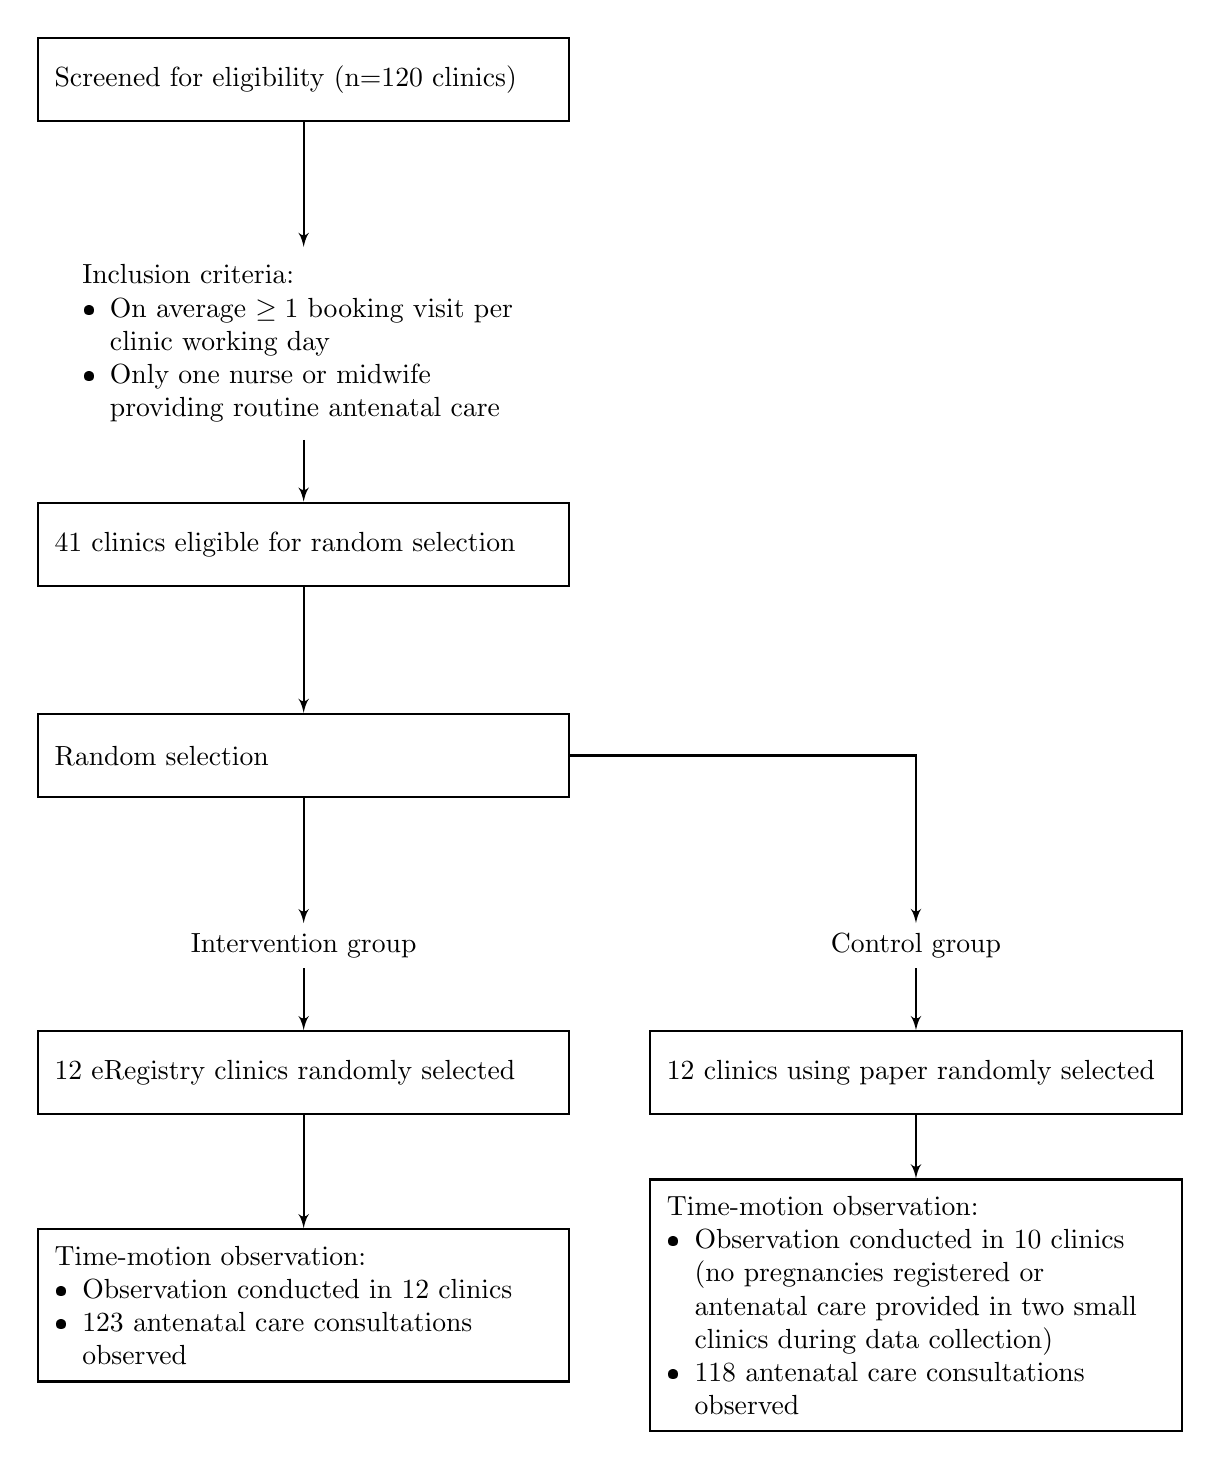
\begin{tikzpicture}[auto,
    block_center/.style ={rectangle, draw=black, thick, fill=white,
      text width=8em, text centered,
      minimum height=4em},
    block_left/.style ={rectangle, draw=black, thick, fill=white,
      text width=16em, text ragged, minimum height=4em, inner sep=6pt},
    block_inclusion/.style ={rectangle, draw=none, thick, fill=none,
      text width=16em, text ragged, minimum height=4em, inner sep=6pt},
    block_noborder/.style ={rectangle, draw=none, thick, fill=none,
      text width=18em, text centered, minimum height=1em},
    block_assign/.style ={rectangle, draw=black, thick, fill=white,
      text width=18em, text ragged, minimum height=3em, inner sep=6pt},
    block_lost/.style ={rectangle, draw=black, thick, fill=white,
      text width=16em, text ragged, minimum height=3em, inner sep=6pt},
      line/.style ={draw, thick, -latex', shorten >=0pt}]
    % outlining the flowchart using the PGF/TikZ matrix function
    \matrix [column sep=10mm,row sep=8mm] {
      % Assessment
      \node [block_assign] (assessment) {Screened for eligibility (n=120 clinics)}; \\
      & {}; \\
      % Inclusion criteria
      \node [block_inclusion] (inclusion) {
          Inclusion criteria:
            \begin{itemize}[leftmargin=*, nolistsep]
              \item On average $\geq 1$ booking visit per clinic working day
              \item Only one nurse or midwife providing routine antenatal care
            \end{itemize}}; \\
      % Included clusters
      \node [block_assign] (included) {
          41 clinics eligible for random selection}; \\
      & \\
      % Random selection
      \node [block_assign] (selection) {
          Random selection}; \\
      & \\
      % Groups
        \node [block_noborder] (i) {Intervention group};
      & \node [block_noborder] (c) {Control group}; \\
      % Allocation
        \node [block_assign] (i_T0) {12 eRegistry clinics randomly selected};
      & \node [block_assign] (c_T0) {12 clinics using paper randomly selected}; \\
      % Observation:
      \node [block_assign] (i_observation) {
        Time-motion observation:
          \begin{itemize}[leftmargin=*, nolistsep]
            \item Observation conducted in 12 clinics
            \item 123 antenatal care consultations observed
          \end{itemize}};
	    & \node [block_assign] (c_observation) {
        Time-motion observation:
          \begin{itemize}[leftmargin=*, nolistsep]
            \item Observation conducted in 10 clinics \\(no pregnancies registered or antenatal care provided in
                  two small clinics during data collection)
            \item 118 antenatal care consultations observed
          \end{itemize}};
      \\
    };% end matrix
    % connecting nodes with paths
    \begin{scope}[every path/.style=line]
      % paths for enrollemnt rows
      \path (assessment) -- (inclusion);
      \path (inclusion)  -- (included);
      \path (included)   -- (selection);
      \path (selection)  -- (i);
      \path (i)          -- (i_T0);
      \path (selection)  -| (c);
      \path (c)          -- (c_T0);
      \path (i_T0)       -- (i_observation);
      \path (c_T0)       -- (c_observation);
    \end{scope}
  \end{tikzpicture}
\end{center}
\end{document}
